% !TEX encoding = UTF-8 Unicode
% !TEX root = project.tex

\documentclass{sig-alternate}
\usepackage{authblk}
\usepackage{url}
\usepackage{subfig}
\usepackage{amsmath}

\begin{document}

%don't want date printed
\date{}

\title{RICE : Review Impact with ConfidencE}

\author{Atri Sarkar}
\author{Bastin Gomez Headmon}
\author{Brian Agala}
\affil{David R. Cheriton School of Computer Science, University of Waterloo}
\affil{\textit {\{a9sarkar,bgheadmo,bagala\}@uwaterloo.ca}}

\maketitle

% Use the following at camera-ready time to suppress page numbers.
% Comment it out when you first submit the paper for review.
\thispagestyle{empty}

\pagenumbering{arabic}

% !TEX encoding = UTF-8 Unicode
% !TEX root = project.tex

\subsection*{Abstract}
The success of open source software systems over the last decade has hugely impacted the way we develop software today. Considering the increasing popularity and participation of the developer community in open source software, maintaining quality is often a daunting task for project owners. In most open source software systems, project owners maintain quality by gatekeeping proposed changes and perform `Change Impact Analysis' of contributions by developers on a daily basis. In this project we develop a tool RICE (Review Impact with ConfidencE), which enables reviewers to easily analyse the impact of a proposed change. The tool mines historical commit data and uses association rule mining to discover the underlying impact a change may cause to the software system. We integrate our tool with the Pull Request UI in GitHub and evaluate its effectiveness on several popular open source projects.

\keywords{Programming tools, association rules, maintenance, data mining, change impact, commit history.}

% !TEX encoding = UTF-8 Unicode
% !TEX root = project.tex

\section{Introduction}
\label{sec:intro}

Over the last decade we have observed a significant shift in the way software is developed. This is driven by big open source organizations such as the Apache and the Mozilla Foundation with generous support from organizations such as Google. Most of the popular software systems such as the Android project, projects in Hadoop and other big data ecosystems, and, dynamic search engine frameworks such as lucene and elasticsearch are a few examples of how open source development has reshaped the way software is developed. Even organizations such as IBM who had traditionally followed a proprietary model recognize the changing landscape and have started to have a strong presence in the open source model as shown by IBM's sponsorship of the Eclipse foundation[7]. As a researcher, it becomes imperative to evaluate our understanding of development processes in light of this changing landscape.

Developers in a typical open source system can fall under two broad non-exclusive categories. In the first category we have the set of developers who are assumed to have a detailed and in-depth knowledge on the design and implementation of the project. They are the developers who have spent significant time with the project, have a higher rate of contribution and have risen the ranks over time to be in a position where they can act as gatekeepers to any change committed in the project. In the second category, we have the rest of the contributors and developers who are not yet in the core group, however, they contribute code to the project's repository by adding new features or by resolving any reported defects. One of the roles which the first category or the core group of developers exercise is the role of a reviewer. This role expects them to exercise the following activities:\\
\begin{enumerate}
\item Review any changes made to the code base by contributing developers to check if the contributions meet the accepted project standards. This role is similar to that of a reviewer in a code-review process.
\item To analyse the impact of the contributions made by developers in the project in general. This includes but is not limited to checking whether the contributing changes are accompanied by required test-cases, whether the contribution runs the risk of breaking existing functionality, or even analysing what needs to be modified to accomplish the intended change. Tasks in this role are usually categorised under Change Impact Analysis (CIA)[2].
\end{enumerate}

In this project, we concern ourselves with this second activity. Based on GitHub data, we have seen that the number of commits in open source projects during peak development periods can reach up to a thousand per day, whereas the number of core developers in a project are usually under one hundred[3]. Under such a scenario, our objective is to assist the reviewer in analysing the impact of a certain change and help him in deciding whether to accept that change or not.\\

\section{Analysing Change Impact}

Changes made to a software system often has the potential of causing collateral side effect or a ripple effect. This ripple effect is measured in terms of the likelihood that a change to a particular set of files may cause problems in the rest of the software [2]. The first step in Change Impact Analysis (CIA) is to look into the list of files that are changed as a part of the change set. Various CIA techniques are used to estimate a list of files that are probably affected by that change. This list of affected files are called Estimated Impact Set (EIS). There are several techniques proposed to generate this EIS and Li et.al provides an exhaustive survey of such techniques[2].

One such technique is based on the hypothesis that impact of a file on another can be measured by looking at how frequently the two files are changed together. The following real world example explains the idea further.

Most software systems today support internationalization (i18n) by which text in user interfaces can be changed easily from one language to another. To implement this, developers are forbidden to hardcode UI texts in English. Instead, the UI files contain a key literal in place of the text which is replaced by the actual language text during runtime. Thus, developers in such systems always need to check-in the language file (which contains the key-value mapping for each language) whenever they add any new field in the UI. In this scenario, we would observe the UI file and the language file to have been checked-in together in the majority of cases. If a new change set comes in for review to the reviewer where he observes only the UI file to have been modified, there is a high chance that the developer would have broken the internationalization functionality of the software.

Our tool generates the list of impacted files (EIS) by mining the historical commit data. We use Top-K association rule mining algorithm to find out the files which have been frequently changed together. Using the algorithm we generate the rules of the form $A \rightarrow B$ where $A$ is the set of files in the change set and $B$ is the EIS set which represents the files impacted due to changes in $A$. Each file in set $B$ is also mapped to a confidence value which gives an estimate of the likelihood of the file being impacted by changes in $A$. The following section gives a brief introduction to Top-K association rule mining algorithm and the process of generating the rules. 

\subsection{Top-K Association Rule Mining}

Association rule mining is the process of discovering associations within items in a set of transactions. A classic application of association rule mining is in supermarkets. Stores look at transaction data of customers and apply association rule mining to generate rules of the kind \{bread\}$\rightarrow$\{milk\} which means that if a customer buys bread, he is very likely to buy milk too.

In our context we can relate items to files and transaction to the change sets. Thus, the objective of association rule mining is formally stated as follows [4] :\\
Let \textbf{I}=$\{a_{1},a_{2},..a_{n}\}$ be a finite set of files in the system. Querying information from the repository data, we can get a set of check-ins \textbf{T}=$\{t_{1},t_{2}..t_{m}\}$ where each check-in $t_{j}\subseteq\textbf{I}$ $(1 \le j \le m)$ represents a single commit in the repository. An itemset is a set of files \textbf{X} $\subseteq$ \textbf{I}. The support of an itemset \textbf{X} is denoted as \textit{sup(\textbf{X})} and is defined as the number of check-ins that contain files in \textbf{X}. An association rule \textbf{X}$\rightarrow$\textbf{Y} is a relationship between two itemsets \textbf{X}, \textbf{Y} such that \textbf{X}, \textbf{Y} $\subseteq$ \textbf{I} and \textbf{X} $\cap$ \textbf{Y}= $\emptyset$. The support of a rule \textbf{X} $\rightarrow$ \textbf{Y} is defined as: 

\begin{equation}
\textit{sup}(\textbf{X} \rightarrow \textbf{Y}) = \textit{sup}(\textbf{X}\cup\textbf{Y}) / |\textbf{T}|.
\end{equation}
 
The confidence of a rule \textbf{X} $\rightarrow$ \textbf{Y} is defined as:

\begin{equation}
conf(\textbf{X} \rightarrow \textbf{Y}) = \textit{sup}(\textbf{X}\cup\textbf{Y}) / \textit{sup}(\textbf{X}). 
\end{equation}

Our objective of mining association rules [5] is to find all association rules in a repository having a support no less than a defined threshold \textit{minsup} and a confidence no less
than a defined threshold \textit{minconf}. These generated association rules measures the impact of a file on another.

Table~\ref{table:checkins_snapshot} shows a snapshot of check-ins in a repository (Table~\ref{table:checkins_snapshot}.a) and the association rules found for \textit{minsup} = 0.5 and \textit{minconf} = 0.5 (Table~\ref{table:checkins_snapshot}.b). Mining associations is done in two steps [5]. Step 1 is to discover all frequent itemsets in the database (itemsets appearing in at least \textit{minsup} $\times$ |T| transactions). Step 2 is to generate association rules by using the frequent itemsets found in step 1. For each frequent itemset \textbf{X}, pairs of frequent itemsets \textbf{P} and \textbf{Q = X - P} are selected to form rules of the form P$\rightarrow$Q. For each such rule \textbf{P$\rightarrow$Q}, if \textit{sup(P$\rightarrow$Q) $\ge$ minsup} and \textit{conf(P$\rightarrow$Q) $\ge$ minconf}, the rule is selected. In our case, we impose an additional constraint that \textbf{P} should be the set of files in the change set proposed by the contributing developer.

\begin{table}[htbp]
  \centering
  \caption{A sample snapshot of check-ins in a repository.}
  \subfloat[Change Sets]{%
    \hspace{.5cm}%
    \begin{tabular}{|c|c|}
        \hline
        \textbf{ID}       & \textbf{ChangeSets}    \\
        \hline
        $t_{1}$       & \{a,b,c,e,f,g\}   \\
        \hline
	$t_{2}$       & \{a,b,c,d,e,f\}   \\
        \hline
	$t_{3}$       & \{a,b,e,f\}   \\
        \hline
	$t_{4}$       & \{b,f,g\}   \\
        \hline
    \end{tabular}%
    \hspace{.5cm}%
  }\hspace{1cm}
  \subfloat[Association Rules]{%
    \hspace{.5cm}%
    \begin{tabular}{|c|c|c|c|}
        \hline
        \textbf{ID}       & \textbf{Rule}       & \textbf{Support} & \textbf{Confidence} \\
        
        \hline
        $r_{1}$        & \{a\} $\rightarrow$ \{b\}       & 0.75 & 1 \\
        \hline
        $r_{1}$        & \{a\} $\rightarrow$ \{c,e,f\}       & 0.5 & 0.6 \\
        \hline
        $r_{1}$        & \{a,b\} $\rightarrow$ \{e,f\}       & 0.75 & 1 \\
        \hline
        ..       & ...       & ... & .. \\
        \hline
    \end{tabular}%
    \hspace{.5cm}%
  }
  \label{table:checkins_snapshot}
\end{table}


Top-K association rule mining [4] is an efficient extension on the traditional A-priori algorithm by Agarwal and Srikanth [5] which mines the \textit{k} strongest association rules found in the itemsets.


\subsection{Pull Requests}


In this project we have built our tool based on the GitHub data and thus it is important to introduce the terminologies involved. Projects in the GitHub system work similar to any other open source project where new, inexperienced, or external developers need to get their changes reviewed by the project owners. In GitHub, this happens through pull requests.\\

\textit{"Pull requests let you tell others about changes you've pushed to a repository on GitHub. Once a pull request is sent, interested parties can review the set of changes, discuss potential modifications, and even push follow-up commits if necessary."} [6] \\

Thus, pull requests contain the set of files changed by the developer. The reviewer reviews the pull request and he has the option to either \textit{approve} or \textit{reject} it. Our RICE tool integrates with the Pull Request UI of GitHub to display an additional list of impacted files along with their confidence value to make this decision process easier for the reviewers.   




% !TEX encoding = UTF-8 Unicode
% !TEX root = project.tex

\section{Related Work}
\label{sec:related}
Do a literature review of the existing work on the topic.

% !TEX encoding = UTF-8 Unicode
% !TEX root = project.tex

\section{Software Setup}
\label{sec:setup}

\begin{figure*}[ht!]
\centering
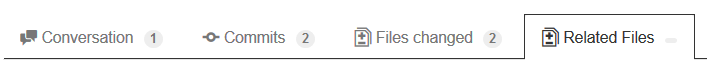
\includegraphics[width=16cm]{NewTabRelatedFiles}
\caption{GitHub pull request page showing the new `Related files' tab}
\label{fig:newTabRelated}
\end{figure*}

\begin{figure*}[ht!]
\centering
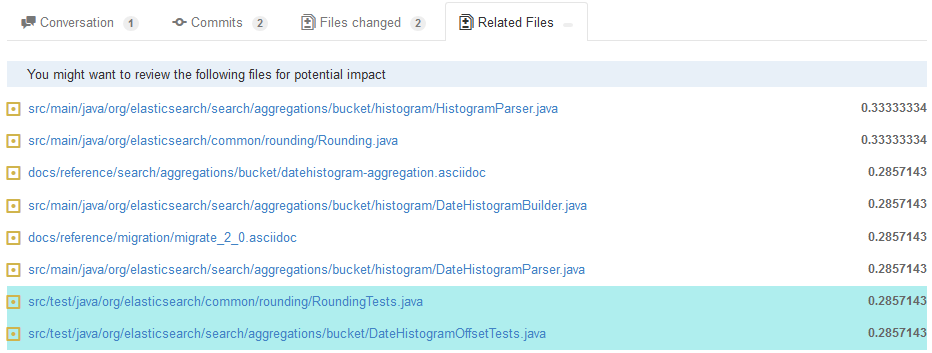
\includegraphics[width=16cm]{RelatedFilesContents}
\caption{`Related files' tab showing files}
\label{fig:relatedFilesContents}
\end{figure*}

\begin{figure*}[ht!]
\centering
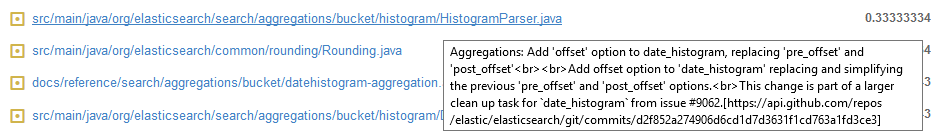
\includegraphics[width=16cm]{MouseOverOfFile}
\caption{Details of the file on performing mouse-over on the hyperlink}
\label{fig:mouseOverOnFile}
\end{figure*}

\begin{figure*}[ht!]
\centering
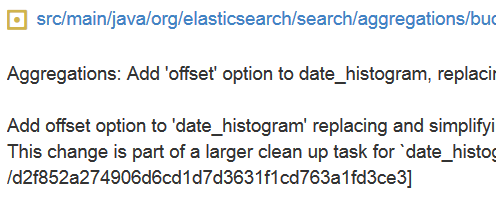
\includegraphics[width=16cm]{ClickOfFileHyperlink}
\caption{Details of the file on clicking on the hyperlink}
\label{fig:clickOnFileHyperlink}
\end{figure*}

The software setup was done on a single laptop having an Intel dual-core i5-4210U CPU running at 1.7 GHz with 8 GB RAM, with Windows 8.1 64 bit operating system. In our setup, we created a Javascript user script which was installed on the Firefox browser using GreaseMonkey add-on~\cite{greasemonkey1,greasemonkey2}. When this script is invoked on a Github pull request page, it adds a new tab named `Related Files' onto the page. Figure~\ref{fig:newTabRelated} shows a screenshot of the webpage showing the new tab. The tab, on opening, sends a REST~\cite{rest} POST~\cite{post_http} request with the all the files from the pull request in its HTTP message body. The REST service, which is deployed on a Glassfish server~\cite{glassfish}, receives the files send from the Github page. The REST service then makes use of the Top-K association rule mining algorithm~\cite{fournier2012mining} to come up with a list of related files and is send back to the Github page, i.e., from where the request was initiated. The Github page will display the results in the 'Related Files' tab. Test files are highlighted in a different color. 

Figure~\ref{fig:relatedFilesContents} shows the contents of the related files tab populated from the REST service output. A confidence value is shown against each file which is obtained from the association rule mining algorithm.

Figure~\ref{fig:mouseOverOnFile} shows what happens when the mouse is hovered over the hyperlink. It shows the reason why the particular file shows up on the related files tab.

Figure~\ref{fig:clickOnFileHyperlink} shows what happens when the hyperlink is clicked. It is the same reason as above, but user can copy the contents if required.



% !TEX encoding = UTF-8 Unicode
% !TEX root = project.tex

\section{Experimental evaluation}
\label{sec:finding}
What did we find in our project

% !TEX encoding = UTF-8 Unicode
% !TEX root = project.tex

\section{Conclusion}
\label{sec:conclusion}
This paragraph will end the body of this sample document. Remember that you might still have Acknowledgments or Appendices; brief samples of these follow.  There is still the Bibliography to deal with; and we will make a disclaimer about that here: with the exception of the reference to the \LaTeX\ book, the citations in this paper are to articles which have nothing to do with the present subject and are used as examples only.


% !TEX encoding = UTF-8 Unicode
% !TEX root = project.tex

\section{Acknowledgments}
This section is optional; it is a location for you
to acknowledge grants, funding, editing assistance and
what have you.  In the present case, for example, the
authors would like to thank Gerald Murray of ACM for
his help in codifying this \textit{Author's Guide}
and the \textbf{.cls} and \textbf{.tex} files that it describes.

%
% The following two commands are all you need in the initial runs of your .tex file to produce the bibliography for the citations in your paper.
\bibliographystyle{abbrv}
\bibliography{project} 

% !TEX encoding = UTF-8 Unicode
% !TEX root = project.tex

%APPENDICES are optional
%\balancecolumns
\appendix
%Appendix A
\section{Headings in Appendices}
The rules about hierarchical headings discussed above for
the body of the article are different in the appendices.
In the \textbf{appendix} environment, the command
\textbf{section} is used to
indicate the start of each Appendix, with alphabetic order
designation (i.e. the first is A, the second B, etc.) and
a title (if you include one).  So, if you need
hierarchical structure
\textit{within} an Appendix, start with \textbf{subsection} as the
highest level. Here is an outline of the body of this
document in Appendix-appropriate form:
\subsection{Introduction}
\subsection{The Body of the Paper}
\subsubsection{Type Changes and  Special Characters}
\subsubsection{Math Equations}
\paragraph{Inline (In-text) Equations}
\paragraph{Display Equations}
\subsubsection{Citations}
\subsubsection{Tables}
\subsubsection{Figures}
\subsubsection{Theorem-like Constructs}
\subsubsection*{A Caveat for the \TeX\ Expert}
\subsection{Conclusions}
\subsection{Acknowledgments}
\subsection{Additional Authors}
This section is inserted by \LaTeX; you do not insert it.
You just add the names and information in the
\texttt{{\char'134}additionalauthors} command at the start
of the document.
\subsection{References}
Generated by bibtex from your ~.bib file.  Run latex,
then bibtex, then latex twice (to resolve references)
to create the ~.bbl file.  Insert that ~.bbl file into
the .tex source file and comment out
the command \texttt{{\char'134}thebibliography}.
% This next section command marks the start of
% Appendix B, and does not continue the present hierarchy
\section{More Help for the Hardy}
The sig-alternate.cls file itself is chock-full of succinct
and helpful comments.  If you consider yourself a moderately
experienced to expert user of \LaTeX, you may find reading
it useful but please remember not to change it.
%\balancecolumns % GM June 2007
% That's all folks!	

\end{document}
